% ドキュメントの設定
\documentclass[a4paper,11pt]{bxjsarticle}

% パッケージのインポート
\usepackage{zxjatype}
\usepackage[ipa]{zxjafont}
\usepackage{graphicx}
\usepackage{listings}
\usepackage{xcolor}

\makeatletter

\def\id#1{\def\@id{#1}}
\def\department#1{\def\@department{#1}}

\def\@maketitle{
\begin{center}
    {\huge データ構造とアルゴリズム演習 \par} %修士論文と記載される部分
    \vspace{1mm}
    {\LARGE 最終課題3 \par}% 論文のタイトル
    {\LARGE レポート \par}
    \vspace{120mm}
    {\Large 所属\ : 情報科学科\ 2年 \par} % 所属
    \vspace{1mm}
    {\Large 学籍番号\ : 19140674 \par} % 学籍番号
    \vspace{2mm}
    {\Large 氏名\ : 久下\ 柾 \par} % 氏名
    \vspace{1mm}
    {\Large 提出日\ : {\today} \par} % 提出部分
\end{center}
\par\vskip 1.5em
}


% ドキュメント開始
\begin{document}

    \maketitle

    \newpage

    % 見出し
    \section{課題3-a}

    図\ref{fig:matrix}の隣接行列をもとにして、世帯同士の関係をグラフで示す。

    \begin{figure}[tbh]
        \begin{center}
            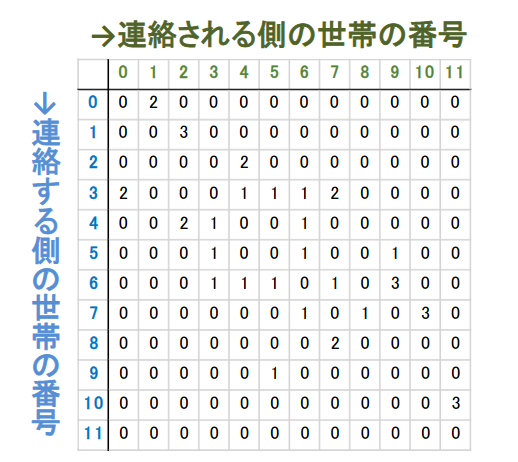
\includegraphics[width=0.6\textwidth]{matrix.png}
            \caption{連絡手段と所要時間を表した隣接行列}
            \label{fig:matrix}
        \end{center}        
    \end{figure}

    この隣接行列を元にグラフを作成すると、図\ref{fig:graph}のように、重み付き有向グラフとして表すことができた。

    \newpage

    \begin{figure}[tbh]
        \begin{center}
            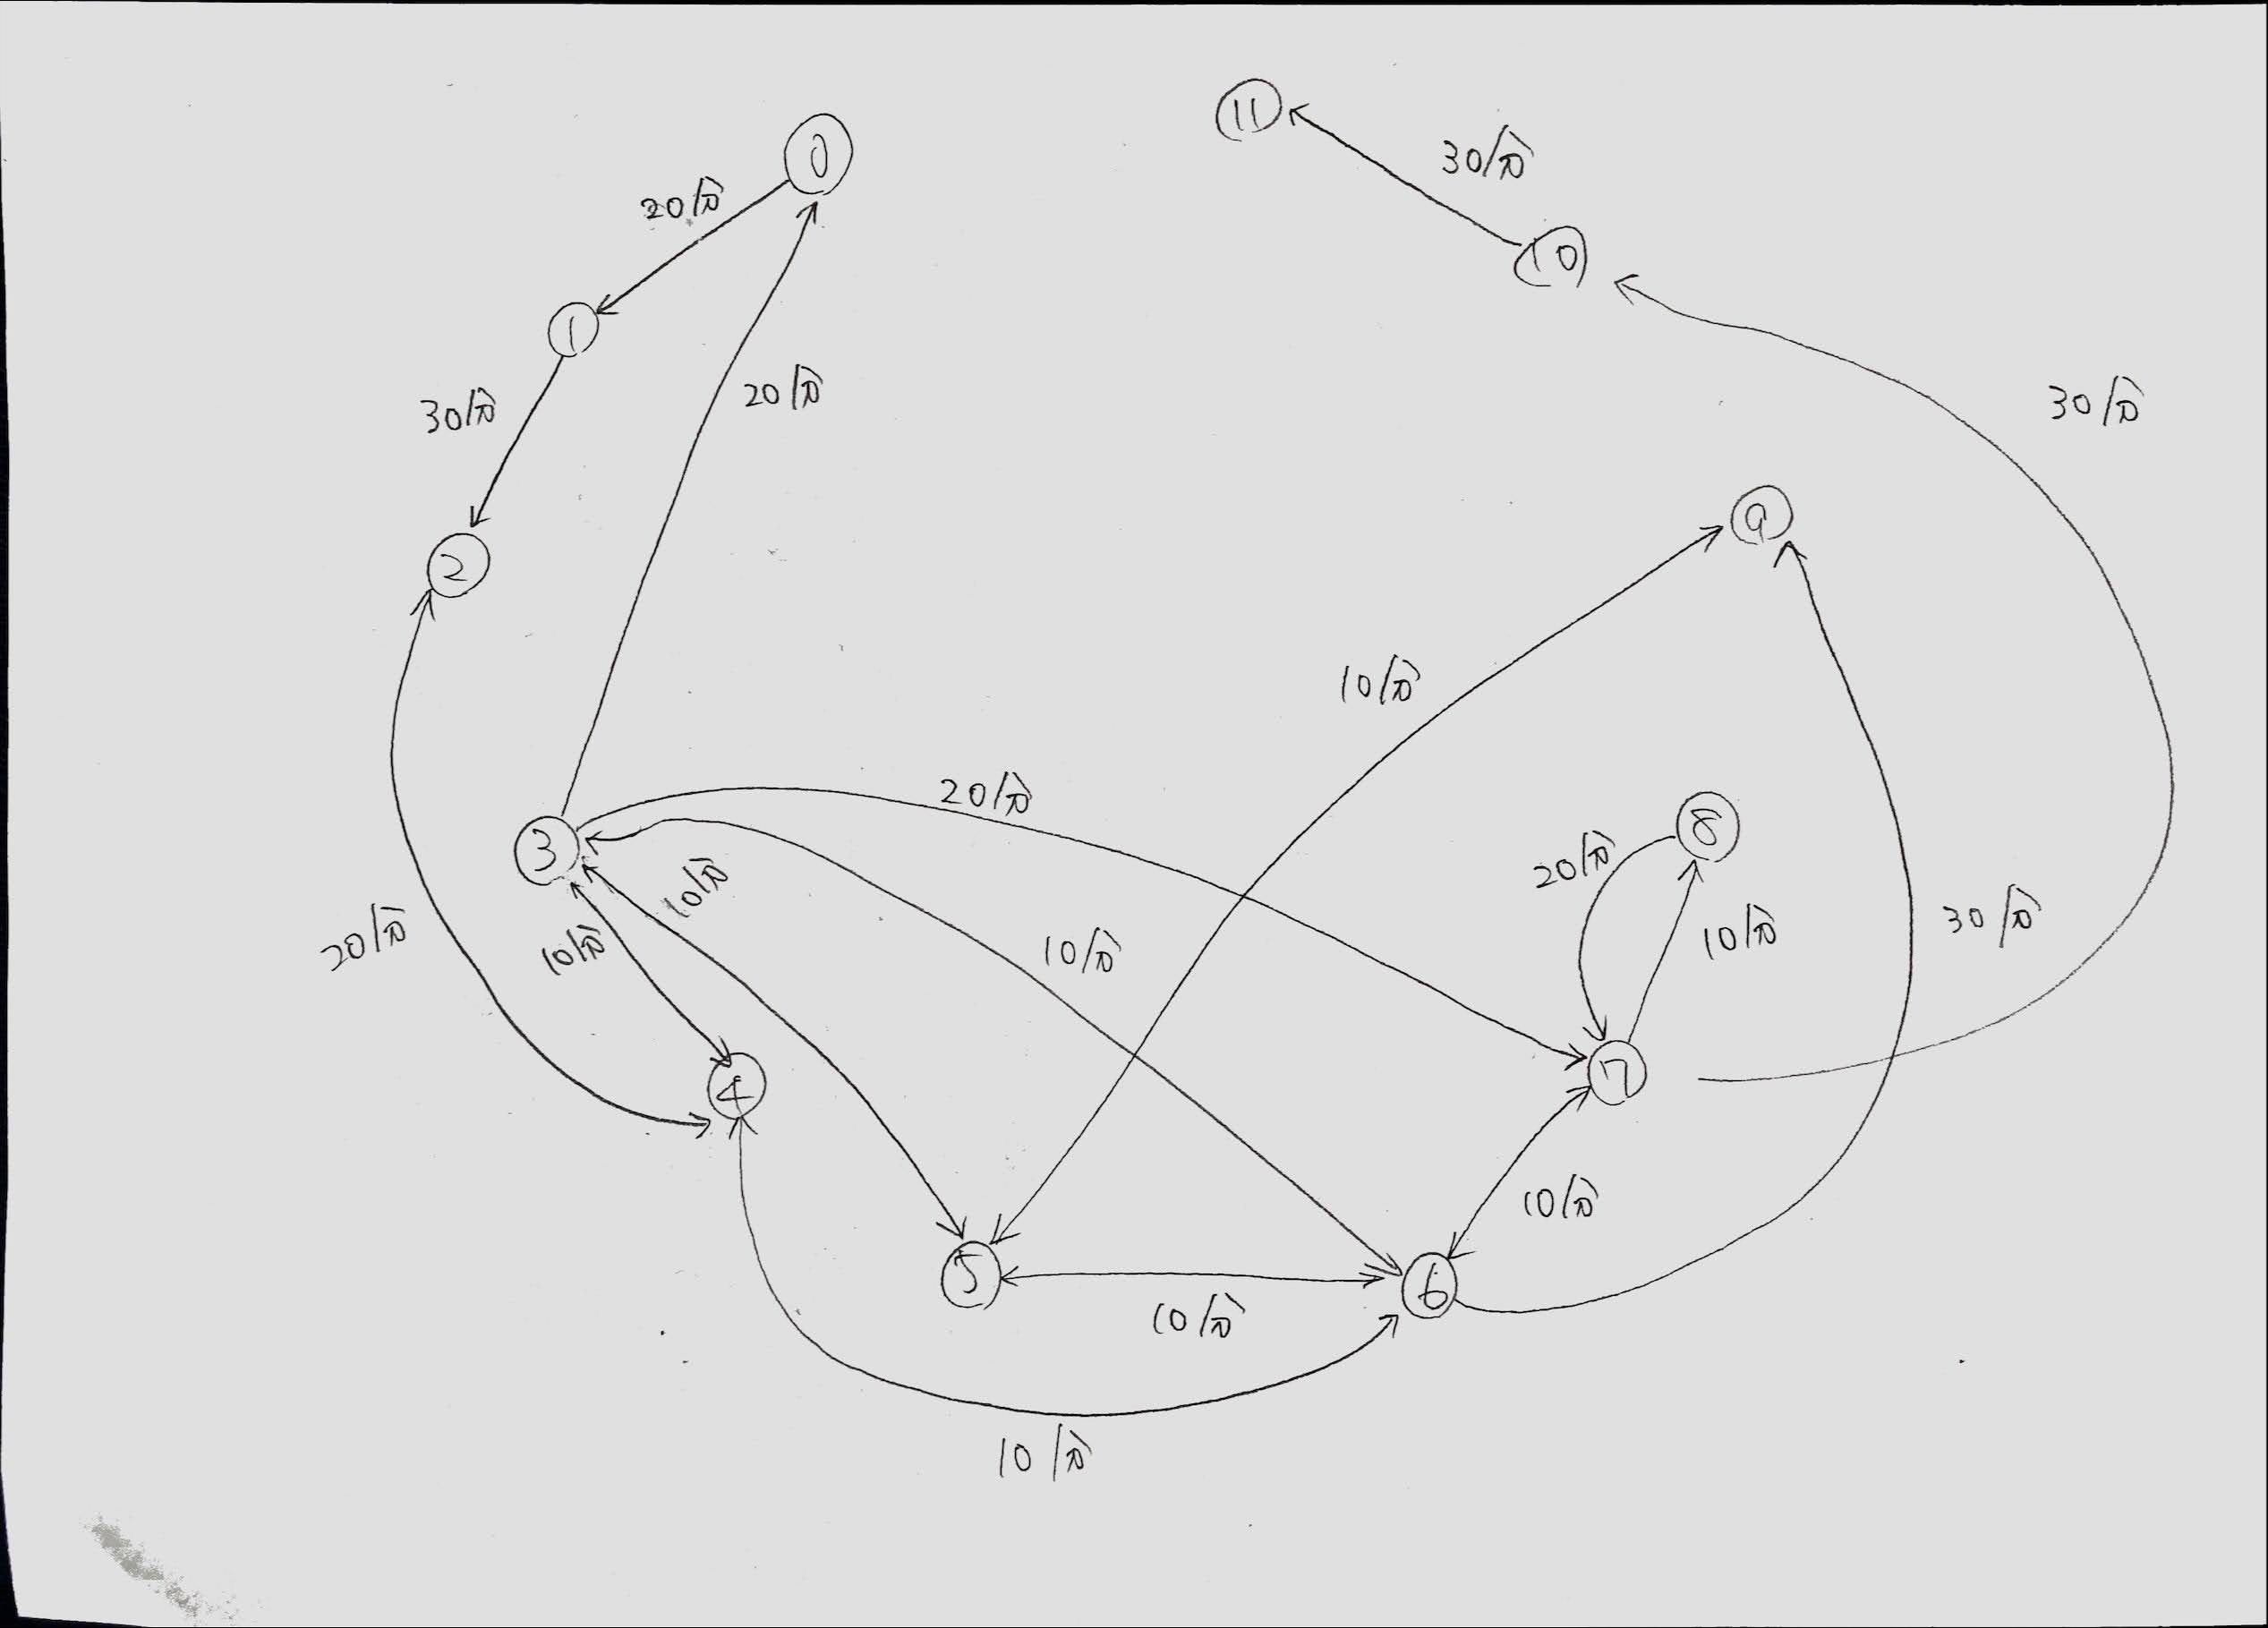
\includegraphics[width=0.9\textwidth]{graph.jpg}
            \caption{町内の関係図のグラフ}
            \label{fig:graph}
        \end{center}        
    \end{figure}



    \newpage

    \section{課題3-b}

    課題3-aで作成したグラフから、最短時間で全員に連絡するために南蛮の世帯を連絡係にするのが適切か求める。
    
    図\ref{fig:matrix}より、以下の点に注意が必要である。

    \begin{itemize}
        \item 3→0→1→2が一方通行
        \item 7→10→11が一方通行かつ11から移動できない
        \item 8は7以外からアクセス不可能
        \item 9のアクセス方法は6→9以外を考慮すべき
    \end{itemize}

    これらの注意点から、10と11は連絡係に選べない。
    また、これは必ずそうでないといけないわけではないが、基本的には同じ場所を複数回通ることは効率が悪くなる。

    これを考慮して総当りで手計算を行うと、図\ref{fig:shortest}の経路が最短であって、連絡係に選ぶべき世帯は9である。

    \begin{figure}[tbh]
        \begin{center}
            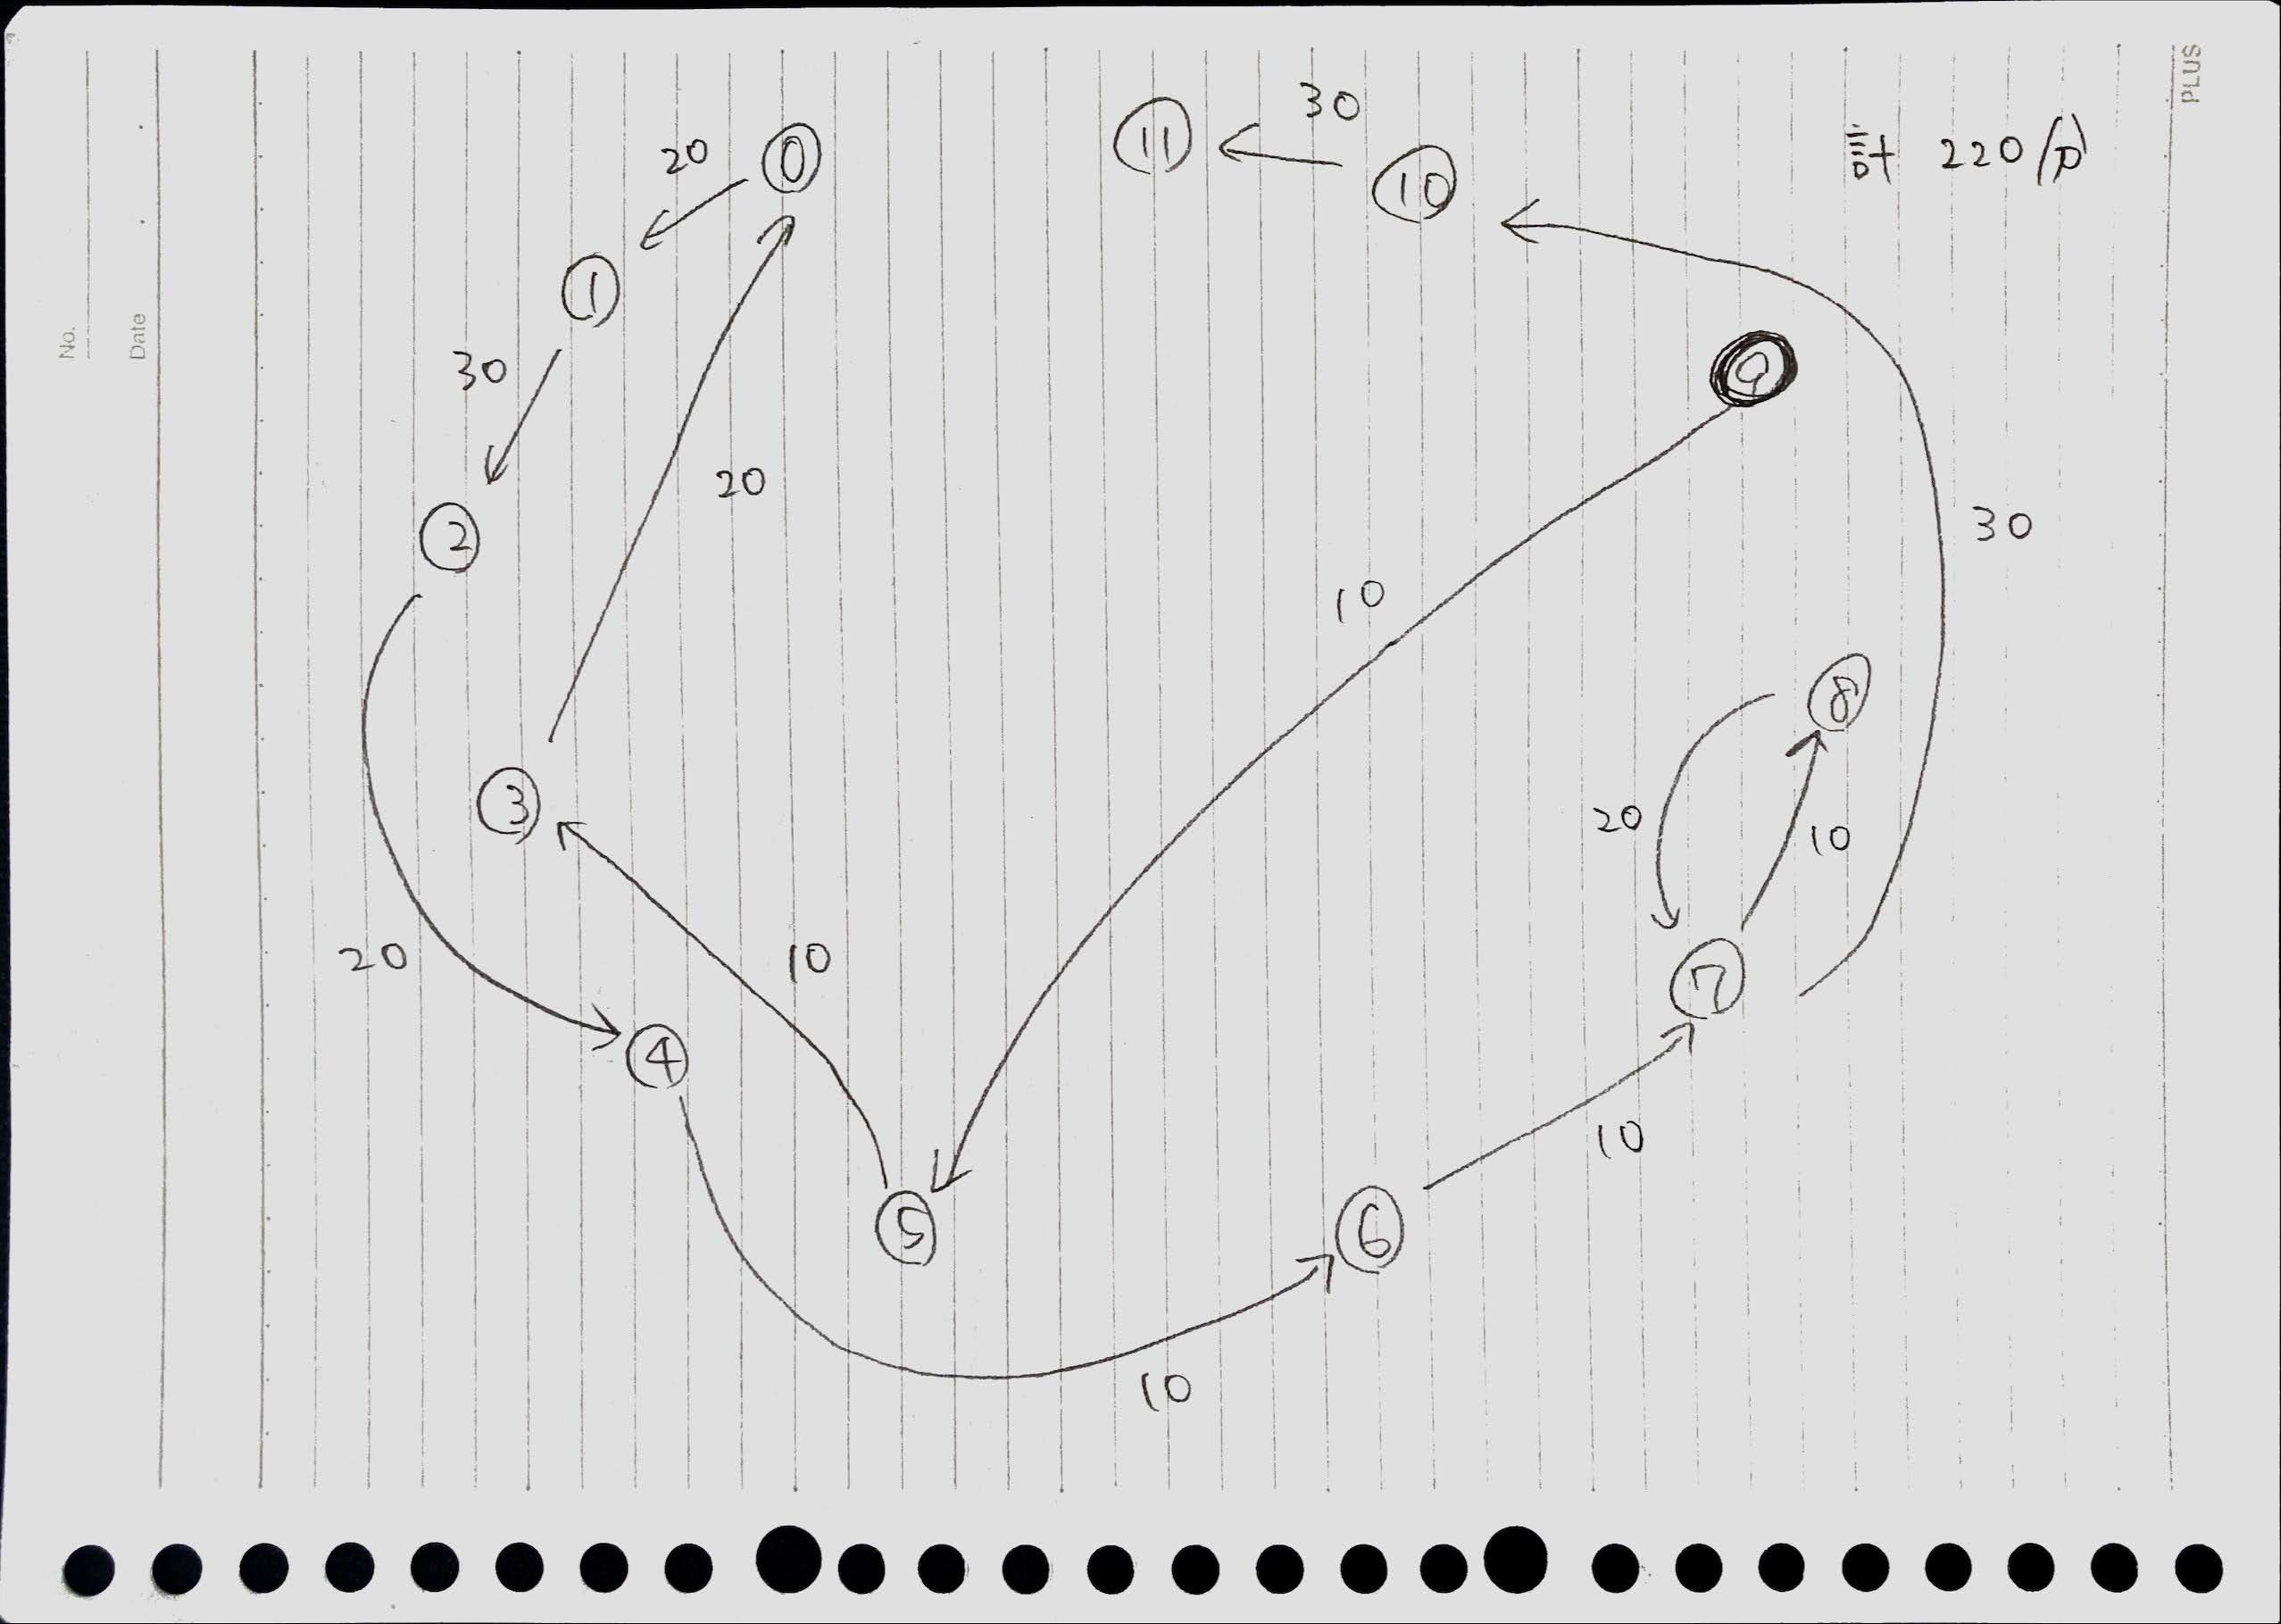
\includegraphics[width=0.9\textwidth]{shortest.JPG}
            \caption{最短経路}
            \label{fig:shortest}
        \end{center}
    \end{figure}

\end{document}